\documentclass[tikz,border=10pt]{standalone}
\usepackage{tikz}
\usepackage{amsmath}

\definecolor{garnet}{HTML}{73000A}
\definecolor{rose}{HTML}{CC2E40}
\definecolor{honeycomb}{HTML}{A49137}
\definecolor{bk70}{HTML}{5C5C5C}

\begin{document}

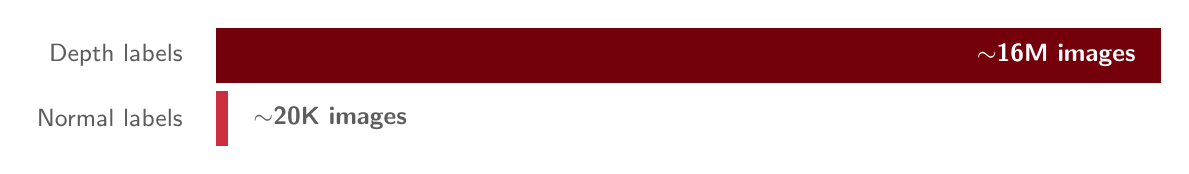
\begin{tikzpicture}

% Depth bar (long)
\fill[garnet] (0, 0.8) rectangle (12, 1.5);
\node[font=\sffamily\small, text=bk70, anchor=east] at (-0.3, 1.15) {Depth labels};
\node[font=\sffamily\small\bfseries, text=white, anchor=east] at (11.8, 1.15) {$\sim$16M images};

% Normal bar (tiny)
\fill[rose] (0, 0) rectangle (0.15, 0.7);
\node[font=\sffamily\small, text=bk70, anchor=east] at (-0.3, 0.35) {Normal labels};
\node[font=\sffamily\small\bfseries, text=bk70, anchor=west] at (0.35, 0.35) {$\sim$20K images};

\end{tikzpicture}

\end{document}
